\chapter[Conclusao]{Conclusão}\

	Por meio do trabalho realizado, foi possível concluir que o processo de renderização como um todo, calculado por meio do tempo de renderização da GPU, terá sempre como complexidade algorítmica uma exponencial para qualquer \textit{shader} (variando somente os coeficientes da função).  Já o processo relacionado ao \textit{vertex shader}, por meio dos experimentos realizados, foi possível perceber que a complexidade algorítmica sempre será linear e o relacionado ao \textit{fragment shader} sempre será um polinômio de segundo grau.

	Analisando a teoria do processo de renderização da \textit{OpenGL} esta conclusão se confirma, pois o programa do \textit{vertex shader} é utilizado para cada vértice (sendo de ordem linear).  O do \textit{fragment shader}, por sua vez, é de ordem do segundo grau, já que seu programa é usado para cada fragmento (sendo uma matriz). Porém este resultado não é tão óbvio, pois se analisarmos o programa do \textit{vertex shader} do Código \ref{vertex_program}, por exemplo, há somente uma atribuição, induzindo a achar que a complexidade é constante. E por meio deste trabalho foi possível perceber que não é.

	\lstinputlisting[language=C, caption = {Exemplo de programa do \textit{vertex shader}}, label = {vertex_program}]{codigos/red_vs.txt} 
	
	Outra contribuição gerada com este trabalho foi quanto à otimização dos \textit{shaders}, em que ao utilizar o processo realizado para a análise da complexidade algorítmica, é possível fazer a comparação entre dois \textit{shaders}, a fim de saber se houve uma otimização ou não. Esta comparação pode ser feita por meio da análise e comparação das funções obtidas, em que pode ser realizada com relação ao processo todo ou especificadamente ao \textit{vertex shader} ou \textit{fragment shader}.

	Pode-se pegar como exemplo as equações relacionadas ao \textit{phong} e \textit{gouraud shaders}. Eles realizam o mesmo cálculo, porém o primeiro faz por fragmento e o segundo, por vértice.  Assim, os coeficientes da equação (Tabela \ref{equacoes}) relacionados ao fragmento do \textit{phong shader} são maiores, e os relacionados ao vértice, menores. 

	A automatização da maior parte deste processo (estrutura para implementação dos \textit{shaders}, média das medições, plotagem e ajuste das curvas), torna-o mais rápido e confiável de ser executado. Ele pode ser resumido na Figura \ref{processo}.

	\begin{figure}[h]
	\centering
		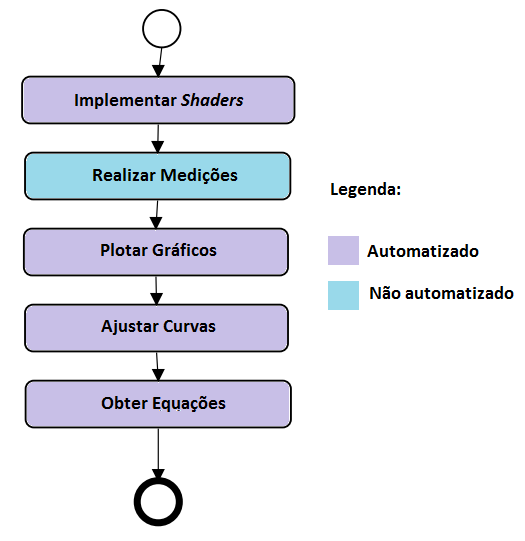
\includegraphics[keepaspectratio=true,scale=0.8]{figuras/processo.png}
	\caption{Processo da Análise de Complexidade Algorítmica.}
	\label{processo}
	\end{figure}
	

	A etapa de Implementar \textit{Shaders} pode ser feita por meio da utilização do projeto implementado, extendendo-se da classe \textit{Shader} e implementando os métodos abstratos, como explicado na Seção \ref{imp}. A Realização das Medições é feita de forma manual, dependendo do \textit{profiler} de GPU adequado para o \textit{device} utilizado. O Plotar Gráficos, Ajustar Curvas e Obter Equações são feitos através do \textit{script} criado.
